\documentclass[xcolor=table]{beamer}
\usepackage{fontspec}
\usepackage{natbib}
\usepackage{multicol,multirow}
\usepackage{gb4e} 
\usepackage[table]{xcolor}
\usepackage{booktabs} 
\usepackage{color}
\usepackage{graphicx}
\usepackage{tikz}
\usetikzlibrary{trees}

\setmainfont[Mapping=tex-text]{SimSun}
\let\sfdefault\rmdefault
%\newcommand{\racine}[1]{\begin{math}\sqrt{#1}\end{math}} 
\newfontfamily\phon[Mapping=tex-text,Ligatures=Common,Scale=MatchLowercase,FakeSlant=0.3]{Charis SIL} 
\newcommand{\ipa}[1]{{\phon \mbox{#1}}} %API tjs en italique
\newcommand{\grise}[1]{\cellcolor{lightgray}\textbf{#1}} 
\newcommand{\ra}{$\Sigma_1$} 
\newcommand{\rc}{$\Sigma_3$} 
\newcommand{\ro}{$\Sigma$}  
\newfontfamily\cn[Mapping=tex-text,Ligatures=Common,Scale=MatchUppercase]{MingLiU}%pour le chinois
\newcommand{\zh}[1]{{\cn #1}}
\XeTeXlinebreaklocale 'zh' %使用中文换行
\XeTeXlinebreakskip = 0pt plus 1pt %
\newcommand{\bleu}[1]{{\color{blue}#1}}
\newcommand{\rouge}[1]{{\color{red}#1}} 
 \newcommand{\marque}[1]{\color{blue}#1} 
 \begin{document}

 \title{嘉绒语支语言的人称范畴}
 \author{Guillaume Jacques  向柏霖}
 \maketitle
  
    \begin{frame} 
 \frametitle{嘉绒语支语言的分布地区} 
 \begin{figure}[H]
\centering
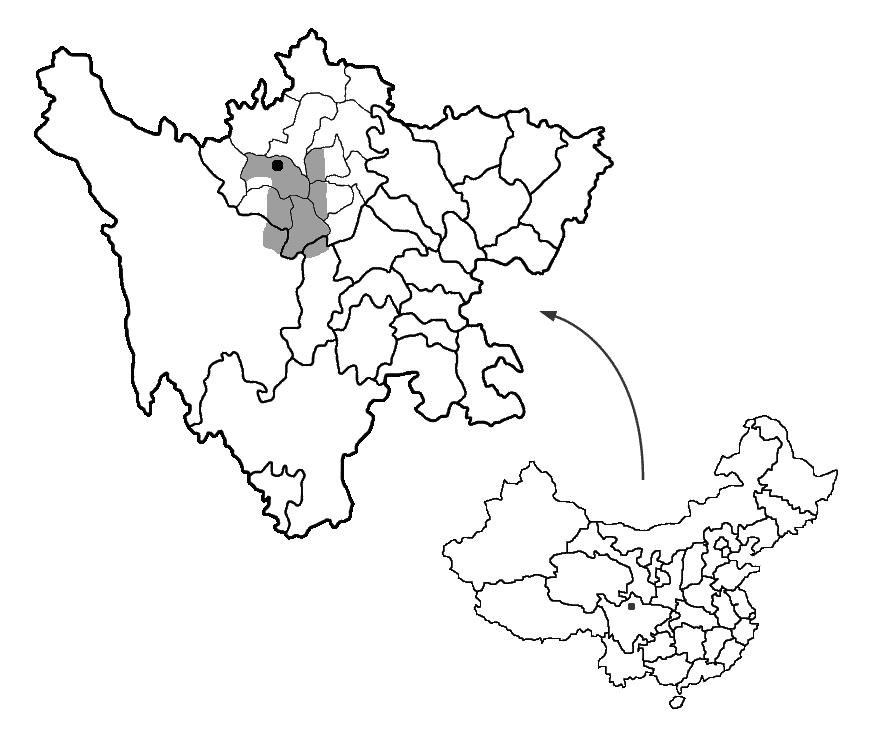
\includegraphics[height=40mm]{carte.JPG}
\end{figure}
  \begin{enumerate}%[<+->]
    \item 嘉绒语
    \begin{enumerate}
 \item 四土话(向柏霖)
 \item 茶堡话(向柏霖)
  \item 草登话
 \item 日部话(龚勋)
  \end{enumerate}
  \item 绰斯甲语(赖云帆)
    \item 道孚语(向柏霖、赖云帆、Antonov)
 \end{enumerate}
  \end{frame}
  
  
     
    \begin{frame} 
 \frametitle{嘉绒语支语言最主要的类型学特征}  
 
 \begin{enumerate}%[<+->]
 \item 多式综合语(双重人称、名词并入) (\citealt{jacques12incorp})
 \item 复杂的动词模板 (\citealt{jacques13harmonization, lai13affixale})
  \item 复杂的词干交替
 \item 丰富的语态标记(包括被动态、使动态、反被动态、应用态、反使动态、反身态等) (\citealt{lai13affixale, jacques14antipassive})
 \item 复杂的复辅音(例如茶堡话 \ipa{lɟɣaʁ} “搭在……上”)
 \item  严格的句法枢纽
  \item 正向/反向标记 (\citealt{jackson02rentongdengdi, jacques10inverse, gongxun14agreement, lai14person})

 \end{enumerate}
   
  \end{frame}   
  
    \begin{frame} 
 \frametitle{人称范畴(不及物动词)}    

\centering
\begin{tabular}{lllllllll} 
\toprule
我 &	\ipa{ɕe-\textbf{a}}  \\
你 &	\ipa{\textbf{tɯ}-ɕe}  \\
他  &	\ipa{ɕe}  \\
\midrule
我俩  & \ipa{ɕe-\textbf{tɕi}}  \\
你俩  &	\ipa{\textbf{tɯ}-ɕe-\textbf{ndʑi}}  \\
他俩  &	\ipa{ɕe-\textbf{ndʑi}}  \\
\midrule
我们  &	\ipa{ɕe-\textbf{j}}  \\
你们 &		\ipa{\textbf{tɯ}-ɕe-\textbf{nɯ}}  \\
他们  &	\ipa{ɕe-\textbf{nɯ}}  \\
\bottomrule
\end{tabular}
   \end{frame}    
  
    \begin{frame} 
 \frametitle{人称范畴(及物动词) 1}      
 
 \begin{exe}
\ex
\gll    \ipa{ʑgrɯ} 	\ipa{ʑo} 	\ipa{ɕɯ-sat-a} 	\ipa{ra}  	\\
一定  强调 去-杀-1单  要 \\
\glt 我一定要去杀他! \marque{1$\rightarrow$3}
\end{exe}
 
  \begin{exe}
\ex
\gll   \ipa{a-wɯ} 	\ipa{cho} 	\ipa{a-ʁi} 	\ipa{ni} 	\ipa{pjɯ-tɯ-sat} 	\ipa{mɤ-jɤɣ} \\
1单:属-爷爷 和 1单:属-弟弟 双 非完成-2-杀 否-可以 \\
  \glt 你不可以杀我爷爷和我弟弟 \marque{2$\rightarrow$3}
  \end{exe}
  
    \begin{exe}
\ex
\gll   \ipa{ji-me} 	\ipa{nɯ} 	\ipa{kɯ} 	\ipa{βɣɯz} 	\ipa{ʁnɯz} 	\ipa{ʑo} 	\ipa{ɕ-pjɤ-sat.} \\
1复:属-女儿 这 做格 獾 两 强调 去-非亲验-杀 \\
  \glt 我们女儿杀了两只獾 \marque{3$\rightarrow$3}
  \end{exe}
  
     \end{frame}      
     
     
      \begin{frame} 
 \frametitle{人称范畴(及物动词) 2}      
\begin{exe}
\ex
  \ipa{tha} 	\ipa{ɣɯ-sat-a} \\
  一会 反-杀-我 \\
  \glt 他要杀我 \marque{3$\rightarrow$1}
\end{exe}

\begin{exe}
\ex
\gll \ipa{nɯ-nɯ-phɣo} 	\ipa{ma} 	 	\ipa{βdaʁmu} 	\ipa{nɯ} 	\ipa{kɯ} 	\ipa{tɯ́-wɣ-sat} 	\ipa{ɲɯ-ŋu} \\
命-为己-逃 连词 女王 这 做格 2-反-杀 亲验-是 \\
\glt 你要逃走,不然女王会把你杀了! \marque{3$\rightarrow$2}
\end{exe}
  
  
\begin{exe}
\ex
\gll     \ipa{pɯ́-wɣ-sat} 	\ipa{ɯ-mɤ-ɕti} 	\ipa{kɯ} \\
完成-反-杀 疑-否-是 疑问 \\
\glt 是不是有人把他给杀了? \marque{3$\rightarrow$3}
\end{exe}
     
     \end{frame}        
     
    \begin{frame} 
 \frametitle{人称范畴(及物动词) 3}      
 
  \begin{exe}
\ex
\gll 
\ipa{tɯrme} 	\ipa{ra} 	\ipa{nɯ-ɕki} 	\ipa{a-mɤ-tɯ-nɤtɯti} 	\ipa{ma} 	\ipa{nɯ maʁ nɤ} 	\ipa{ta-sat} \\
人 复 3复-于格 未然-否-2-到处说 连词 不然 1$\rightarrow$2-杀 \\
 \glt 你不要到处跟人说,不然我就会杀你 \marque{1$\rightarrow$2}
 \end{exe}
 
 \begin{exe}
\ex
\gll     \ipa{tɕhindʐa} 	\ipa{kɯ-sat-a} 	\ipa{ɲɯ-ra}  	\\
为什么 2$\rightarrow$1-杀-1单 亲验-要 \\
\glt (渔夫对魔鬼说)“为什么要杀我?” \marque{2$\rightarrow$1}
\end{exe}
 
  
     \end{frame}    
     
         \begin{frame} 
 \frametitle{人称范畴(及物动词)}      
     
 \centering
\begin{tabular}{llllll}
&     1 & 2 & 3 &3'\\
\toprule
 1 &\grise{} &\ipa{ta-sat} & \ipa{sat-a}\\  
 2 &\ipa{kɯ-sat-a}&\grise{}  &  \ipa{tɯ-sat}\\  
 3 & \ipa{\rouge{ɣɯ}-sat-a}&  \ipa{tɯ́-\rouge{wɣ}-sat}&\grise{}   &\ipa{sat} \\
  3'&  &&  \ipa{\rouge{ɣɯ}-sat}\\
  \bottomrule
\end{tabular}
\end{frame} 
          
          
 \begin{frame} 
 \frametitle{词干交替}      
     
     \centering
 \begin{tabular}{llllll}
&     1 & 2 & 3 &3'\\
\toprule
 1 &\grise{} &\ipa{ta-mto} & \ipa{\bleu{mtam}-a}\\  
 2 &\ipa{kɯ-sat-a}&\grise{}  &  \ipa{tɯ-\bleu{mtɤm}}\\  
 3 & \ipa{\rouge{ɣɯ}-mto-a}&  \ipa{tɯ́-\rouge{wɣ}-mto}&\grise{}   &\ipa{\bleu{mtɤm}} \\
  3'&  &&  \ipa{\rouge{ɣɯ}-mto}\\
  \bottomrule
\end{tabular}
     
\end{frame}    

    \begin{frame} 
 \frametitle{双数和复数后缀}      

\begin{exe}
\ex 
\gll \ipa{ɯ-pi} 	\ipa{ni} 	\ipa{kɯ} 	\ipa{pa-mto-ndʑi}  \\
3单:属-哥哥 双 做格 完成:3$\rightarrow$3'-看-双 \\
\glt 两个哥哥看见了(那件事) \marque{3双$\rightarrow$3}
\end{exe}

\begin{exe}
\ex 
\gll \ipa{tɤ-pi} 	\ipa{ʁnaʁna} 	\ipa{ʑo} 	\ipa{pɯ́-wɣ-sat-ndʑi} 	\ipa{ɲɯ-ŋu} \\
不定:属-哥哥 两个 强调 完成-反-杀-双 亲验-是 \\
\glt (他们/他)把两个哥哥杀了 \marque{3$\rightarrow$3双}
\end{exe}

\begin{exe}
\ex 
\gll
\ipa{nɤ-pi} 	\ipa{ni} 	\ipa{kɯ} 	\ipa{tɤ́-wɣ-nɯmɢla-a-ndʑi} 	\ipa{ɕti} \\
2单:属-姐姐 双 做格 完成-反-跨-1单-双 是 \\
\glt 你的两个姐姐从我身上跨过去了 \marque{3双$\rightarrow$1单}
\end{exe}


\end{frame}    


         \begin{frame} 
 \frametitle{双数和复数后缀}      

 \centering
 \resizebox{\columnwidth}{!}{
\begin{tabular}{lllllllll}
&     1 & 2 & 3单  &3双 & 3复 &3'\\
\toprule
 1 &\grise{} &\ipa{ta-sat} & \ipa{sat-a}&\ipa{sat-a-\bleu{ndʑi}}&\ipa{sat-a-\bleu{nɯ}}&\\  
 2 &\ipa{kɯ-sat-a}&\grise{}  & & \ipa{tɯ-sat}\\  
 3单 & \ipa{\rouge{ɣɯ}-sat-a}&  &\grise{}&\grise{}&\grise{}   &\ipa{sat} \\
  3双 & \ipa{\rouge{ɣɯ}-sat-a-\bleu{ndʑi}}&  \ipa{tɯ́-\rouge{wɣ}-sat}&\grise{}&\grise{}&\grise{}   &\ipa{sat-\bleu{ndʑi}} \\
   3复 & \ipa{\rouge{ɣɯ}-sat-a-\bleu{nɯ}}&   &\grise{}&\grise{}&\grise{}   &\ipa{sat-\bleu{nɯ}} \\
  3'&  &&  \ipa{\rouge{ɣɯ}-sat}&\ipa{\rouge{ɣɯ}-sat-\bleu{ndʑi}}&\ipa{\rouge{ɣɯ}-sat-\bleu{nɯ}}&\\
  \bottomrule
\end{tabular}}
\end{frame} 

\begin{frame} 
 \frametitle{绰斯甲语和道孚语}      
 
\citet{jacques14rtau} 
 
 \begin{table}
\caption{\ipa{f-kʰʚ} 给}
\centering \label{tab:give}
\begin{tabular}{|c|c|c|c|c|}  
 \cline{1-4}
 &  	1   &  	2  &  	3  \\  
\cline{1-4}
 1s  &   \grise{}      &  	\multirow{2}{*}{\ipa{tə-kʰʚ}}  &  	\ipa{tə-kʰow}  \\  
\cline{4-4}1p  &   \grise{}	    &  & \ipa{tə-kʰõ}  \\  
\cline{2-4}2 &     \multirow{2}{*}{\ipa{tə-\rouge{f}kʰõ}}    &   \grise{ } &  	\ipa{tə-kʰe}\\  
\cline{3-4}3 &     & \multicolumn{2}{c}{ \ipa{tə-\rouge{f}kʰʚ} } \vline \\  
\cline{1-4}
\end{tabular}
\end{table}
\end{frame} 



   \begin{frame} 
 \frametitle{参考目录}
 \tiny
 \bibliographystyle{unified}
\bibliography{bibliogj}
 \end{frame}

\end{document}